\documentclass[
  journal=Hypatia,
  manuscript=Musing,  %% article (default), rescience, data, software, proceedings, poster
  layout=preprint,  %% preprint (for submission) or publish (for publisher only)
  year=2026,
  volume=,
]{extra/joas}
%\doi{10.13140/RG.2.2.27723.66085}
%\received {1 Sep 2025}
%\revised  {1 Dec 2025}
%\accepted {10 Dec 2025}
%\published{20 Dec 2025}
%\editor{Joanna Thorne}
%\reviewers{Anonymous reviewers}

\usepackage{biblatex}
\usepackage{xeCJK}
\usepackage{microtype}
\usepackage{cleveref}
\usepackage{hyperref}
\usepackage{csquotes}
\MakeOuterQuote{"}
\usepackage{endnotes}
\renewcommand{\abstractname}{Abstract}
\renewcommand{\figurename}{Figure}
\renewcommand{\tablename}{Table}
\renewcommand{\refname}{References}
\addbibresource{references.bib}
\DeclareNameAlias{sortname}{family-given}
\DeclareNameAlias{default}{family-given}
\usepackage{lineno}
\nolinenumbers

\title{Predictive coding and a pair of red shoes: a materialist account of gender identity}

\author{Anonymous Author}
%\affiliation{Division of Ecology and Evolutionary Biology, School of Biological Science, University of Reading, Whiteknights, Reading, RG6 6EX, United Kingdom}
%\email{j.sun@pgr.reading.ac.uk}
%\date{12/01/2026}

\keywords{Gender identity, philosophy of biology, philosophy of mind, sex/gender distinction}

\begin{document}

\maketitle

\begin{abstract}
This paper proposes that gender identity emerges through the brain's predictive coding mechanism. Under this framework, the brain updates its internal self-model to minimise prediction errors arising from the incongruence between embodied raw feelings -- stemming from body representation, sensory processing (e.g., in autism), or social trauma -- and assigned gender categories. This model resolves the tension between biological reality and social construction, characterising gender identity not as a metaphysical essence but as a constructed self-model. Finally, the political implications are discussed, in which, specifically, I take my own gender identity as an example in the discussion. This article ultimately argues that adopting a predictive coding framework offers a materialist explanation for transgender experiences -- one that validates our raw feelings without essentialising them.
\end{abstract}

\addcontentsline{toc}{section}{Abstract}

\section{Introduction}

The contemporary intellectual landscape surrounding gender is dominated by two contending theoretical frameworks: biological essentialism and post-structuralist queer theory. The former frequently posits ``gender identity'' as an inherent essence \parencite{APA2015Guidelines, NHS2022Gender}, anchoring social identity in the brain, a view supported by some neurologists. Conversely, post-structuralism, exemplified by the work of \textcite{Butler1990Gender}, approaches gender as a socially constructed and performative phenomenon, denying the objective understanding of pre-discursive biological reality. However, while essentialism struggles to account for neuroplasticity and the complexity of abstract concepts, strict social constructionism often fails to integrate the material reality and our embodied raw feelings. In this article, I propose a synthesis using the framework of predictive coding. I argue that "gender identity" is neither a genetic inevitability nor a purely linguistic performance, but a cognitive solution generated by the brain to resolve prediction errors. To establish this, I will first dismantle the definition of "biological sex," demonstrating its scientific redundancy when applied beyond gametes. Subsequently, I will review neurological evidence to show how the predictive coding theory integrates our embodied raw feelings and social norms, to construct a gendered self-model.

\section{Dismantling "sex"}
In this section, I will illustrate that the definition of the so-called "biological sex" involves the fallacy of begging the question and contradicts Occam's razor as a scientific redundancy. This argument is necessary for further discussion because many scientific models I will discuss repeat this fallacy when explaining gender identity. In this article, I use ``phenotypic sex'' as an alternative to the conventional term ``biological sex,'' because the academic biological definition of sex is strictly confined to the types of gametes \parencite{Lehtonen2014Gamete, Goymann2023Biological, Hurst1996There, Griffiths2025Biology}, and its determination mechanisms are homologous among the entire vertebrate lineage \parencite{Bellott2017Avian, Graves2010Homologies, Smith2007Bird}. Different clades have developed different sex chromosomes, genitals, and sexual dimorphic characteristics in the evolutionary history. These characteristics are dynamically shaped by sexual selection. Genitals can change extremely fast in some groups, e.g., some ducks \parencite{Brennan2007Coevolution, Orbach2018Evolution}, which is not different from other sexual dimorphic traits. The phenotypic sex (so-called ``biological sex'') is merely an arbitrarily organised subset of sexual dimorphic traits. Its scope is unjustified. \textcite{Zieminska2022Toward} proposed the so-called "five layers of sex," namely sex chromosomes, gonads, internal sex organs, external genitals, and secondary sex characteristics. From an evolutionary perspective, the sexual dimorphism of height possesses no essential difference from that of sex chromosomes, genitals, or secondary sex characteristics. The difference lies solely in the degree of overlap; height exhibits significantly greater overlap than genitalia. This is a quantitative difference rather than a fundamental one. They are all adaptive traits that promote the rate of reproduction success. Then why are tall "women" or short "men" not considered "intersex?" In what way are the five layers different from other sexual dimorphic traits? This is a typical instance of begging the question. As an instrumental proxy of gametic sex, its functions can be replaced by sexual dimorphism or some specific sexual dimorphic traits, therefore framing it as a scientific redundancy. Moreover, using the same term "sex" for gametes and an arbitrary subset of sexual dimorphic traits wrongly implies that they are more closely related than other sexual dimorphic traits. It should be named "strongly sexual dimorphic traits" rather than "sex."

Secondary sexual characteristics are sometimes considered part of phenotypic sex (e.g., \cite{Zieminska2022Toward}). However, intersex conditions are practically diagnosed only by their gonads and genitals, not the whole range of "sex." Individuals with gynaecomastia are not considered intersex. For individuals with gynaecomastia who self-identify as male, medical treatment for their breasts is also to ``make their body consistent with their gender identity,'' while it is not considered a "gender-affirming surgery." What does the component "sex" mean in this term? \textcite{AMA2021Advancing} define "intersex" as "individuals whose reproductive organs and anatomy (e.g., primary sex characteristics, hormones, chromosomes, etc.) do not align with medically defined and socially expected notions of male and female." Why aren't individuals with polycystic ovaries syndrome (PCOS) "intersex," since their hormones do not align with typical male or female phenotypes. The definition of phenotypic sex and related terms are not only unjustified, but also blurred, nebulous, and unstable, even sometimes self-contradictory. 


\section{Neurology on Gender Identity}
In this section, I will demonstrate that the idea of an "innate," or "inherent" gender identity is groundless and directly contradicts many biological laws.

\textcite{APA2015Guidelines} defines "gender identity" as "a person's deeply felt, inherent sense of being a girl, woman, or female; a boy, a man, or male; a blend of male or female; or an alternative gender." \textcite{NHS2022Gender} defines it as "a way to describe a person's innate sense of their own gender, whether male, female, or non-binary."

It is untenable that we have an innate feeling about "gender" because it is a social construct. From a physicalist and reductionist perspective, one's gender identity is the product of a specific physical state of their brain, involving the connection patterns of neurons. Theoretically, the human brains could be initialised in this state as long as there are enough genes about it. However, this claim is too \textit{ad hoc}. As an analogy, infants have the sucking reflex without knowing what a ``breast'' is. Innately encoding a ``gender identity'' is more useless than encoding a ``breast.'' The latter would allow infants to recognise breasts innately, distinguish what should and should not suck, and avoid sucking on harmful things. Therefore, an innate ``gender identity'' is less probable than an innate concept of breasts. Moreover, using so many genes to encode such a metaphysical, abstract concept is biologically inefficient and impractical, without reasonable selection pressure. In contrast, evolving a brain with high neuroplasticity to learn abstract concepts is far more reasonable.

%By definition, it clearly falls under the concept of "narrative identity" or "narrative self", specifically, "self-concept," which is defined as the "conscious beliefs about the self that are descriptive or evaluative" \parencite{Fanti2024Dual}. In contemporary psychology, cognitive science and philosophy of mind, there is a broad consensus that narrative identity is essentially a posteriori. It is formed through the integration and interpretation of personal life experiences and is deeply influenced by sociocultural frameworks \parencite{Fanti2024Dual}. Therefore, claiming that gender identity is a priori or innate creates a profound philosophical contradiction.

Many neuroscience research claiming an ``innate gender identity'' involves circular reasoning and explanatory gaps. They used the brains of individuals who conform to assigned gender roles (so-called ``cisgender'') as ``male brains''/``female brains.'' However, without human society and culture, this would just be a sexual dimorphic neurological trait, but not ``male'' or ``female.'' If it could be considered ``male'' or ``female,'' tall/short individuals would also be considered ``male height'' and ``female height,'' so would fat/thin individuals, because they are also sexual dimorphic characteristics \parencite{Wells2007Sexual}. Additionally, research shows that almost no one's brain is entirely "male" or entirely "female"; the vast majority of people have a mixture of "typical male" and "typical female" characteristics \parencite{Baxendale2025Brain, Joel2015Sex}.

Primatologist Frans de Waal even claimed that ``primates are born with a gender identity'' because their behaviour does not conform to the statistical typic for their phenotypic sex, such as the phenotypically female chimpanzee Donna, who occupies territory and fights with others~\parencite{DeWaal2022Different, Morin2022Frans}. However, nobody has ever asked ``Hi, Donna, what is your gender identity?'' De Waal's claim is effectively saying that gender identity is a behavioural characteristic of animals. Animals exhibit sexual dimorphic behaviour, while equating "aggression" with "male identity" is not only anthropomorphism, but also a logical leap. From an evolutionary perspective, "aggression" offers a survival advantage, but an abstract concept like "I am a male chimpanzee" would have been entirely unprofitable and highly energy-intensive for animals without language.

Discomfort with a specific body morphology starts from an early age, reported by some transgender individuals, may indeed stem from internal body representation, which was revealed by some neuroscience studies \parencite{Case2017Altered, Lin2014Neural, Ramachandran2008Phantom}. However, according to the sex/gender division, a preference for a specific body morphology should not be considered "gender identity" itself. This is a category error.

The reason they are interpreted within the framework of ``gender'' is a product of society and culture. The sex \textit{sensu stricto} is strictly confined to the gametes in biology \parencite{Lehtonen2014Gamete, Goymann2023Biological, Hurst1996There, Griffiths2025Biology}, and its determination mechanisms are homologous among the entire vertebrate lineage \parencite{Bellott2017Avian, Graves2010Homologies, Smith2007Bird}. Different clades have developed different sex chromosomes, sex organs, and sexual dimorphism in the evolutionary history. These characteristics are dynamically shaped by sexual selection. The phenotypic sex (so-called ``biological sex'') is merely a socially organised set of sexual dimorphic traits from all of them. The boundaries are very blurry, and the standards are inconsistent and unstable. For example, breasts are sometimes considered part of phenotypic sex (e.g., in gender-affirming surgery), but not when determining intersex conditions. Intersex individuals are judged only by their genitals; individuals with gynaecomastia are not considered intersex. For individuals with gynaecomastia who self-identify as male, medical treatment for their breasts is also to ``make their body consistent with their gender identity,'' which therefore should also be considered a gender-affirming surgery. It is shaped by the sociocultural construct that why we understand body representation incongruence about some parts as ``gender dysphoria,'' while other parts as ``body dysmorphic disorder'' or ``body integrity identity disorder.''

A nature-nurture co-operation hypothesis is strongly supported by the aforementioned neurological studies. \textcite{Case2017Altered} suggest an innate multimodal body representation but acknowledge that culture and experience can shape it, making the ``innate'' vs. ``acquired'' line blurry. \textcite{Lin2014Neural} revealed that transgender individual's brains showed high connectivity between the body representation areas and visual/auditory processing areas. They suggest this means transgender individuals are ``integrating massive visual and auditory cues to shape their body image,'' and transgender people's ``distinct neural network of body representation can be coterminal to genetic constitution, developmental factors and learned experience in their life.'' This means that our brains use learned socio-cultural knowledge to interpret a vague, underlying discomfort into a specific, socially coherent narrative. Evolution may have encoded certain raw feelings about body representation, personality, or other traits. Nonetheless, these studies, as well as similar neurological studies, mainly focus on ``typical,'' early-onset transgender individuals. In contrast, studies focus on ``atypical'' transgender or non-binary individuals are relatively rare. \textcite{Bonazzi2025Gender} demonstrate the significant relevance between autism and transgender identity. The neurological heterogeneity between body representation incongruence and autism implies that ``transgender'' people do not share a biological essence.

According to the predictive coding framework, the human brain functions as a continuous prediction engine, leveraging past knowledge and internal models to efficiently anticipate sensory data and thereby minimise unexpected outcomes \parencite{Clark2013Whatever}. \textcite{Tacikowski2020Fluidity} demonstrated that the perceptual illusion of owning a phenotypic opposite-sex body causes a dynamic, robust, and automatic shift in gender identity, characterized by a more balanced subjective identification with both genders, updated implicit self-associations, and reduced gender-stereotypical beliefs regarding one's own personality. If an individual has a sensory processing variation (e.g., the breast feels ``alien''), this creates a prediction error. The brain can resolve this error by updating its ``self-model.'' If the social environment offers a category (``Transgender Man'') that explains this feeling, the brain adopts this identity to minimise the error. Similarly, as demonstrated by \textcite{Clausen2021Action}, footstep sounds can modulate gender identity and the sense of self-group relation in cisgender participants. Therefore, ``gender identity'' is shaped through updating our self model to resolve the continuous prediction failure in multiple aspects because one or many of our raw feelings are incongruence with gender categories. Body representation incongruent people's raw feeling might be ``this body part isn't mine.'' Autistic people's raw feeling might be ``the arbitrary gender norm is hard to conform and makes me uncomfortable.'' Some people with gender non-conforming personalities and behaviours might feel ``I dislike the personality/temperament externally forced on me.'' Other transgender individuals might develop their gender identity through personal history. The gender construct ties disparate causes together and make us interpret them as ``This means I am a girl/boy/man/woman/non-binary person.'' ``Gender identity'' is therefore not an internal essence, but a post-hoc rationalisation, a ``conceptual chimaera.'' It connects a pre-linguistic raw feeling with a purely socially constructed category of identity. Then it claims this connection is ``natural,'' using the raw feeling to legitimise a social construct.

Therefore, we must distinguish between the biological causes and the psychological explanation. The former are continuous, mosaic, and low-level biological traits. The latter is a discrete, high-level semantic label recruited by the brain's predictive machinery to make sense of the former within a specific cultural framework. Confusing them is the fundamental error of gender essentialism.

To elucidate the mechanisms by which a "gender identity" is formed without resorting to essentialism, this narrative incorporates a detailed autobiographical case study (\hyperref{app:case-study}). It is necessary to explicitly acknowledge the epistemological limitations of this approach. As a subjective account of a single individual (N=1), this autobiography does not claim to generate universal statistical data or prove a biological rule on its own. Instead, it is offered as supplementary evidence to the broader theoretical and scientific argument.

%If we were to judge intersex conditions in humans as we do in birds, based on external genitalia alone, then most birds (except for a few groups like ducks, whose males have a penis) have the same external genitalia (a cloaca), so they should not have the concept of ``intersex'' at all. Some ornithologists classify birds as intersex based on mixed plumage colour \parencite{Choudhary2024Intersex}, but feathers' relationship to reproduction is less direct than that of mammalian breasts (used for lactation). Their function is more like our body hair, Adam's apple, beard, and facial features, which are purely for attracting mates and not physiologically related to reproduction.

%If birds' mixed plumage can be used to classify intersex, then individuals with gynaecomastia should also be intersex. The neutral neurological traits related to an individual's personality, behaviour patterns, and body representation, which make them more likely to form a specific gender identity when interacting with current social gender norms, are also a form of sexual dimorphism and have a significant statistical correlation with gametes (sex \textit{sensu stricto}). Thus, theoretically, they should also be part of ``phenotypic sex.''

%If we apply the standard for birds to ourselves, an individual whose certain sexually dimorphic traits differ from the statistical norm for their gametic sex could be considered intersex. Then, transgender people whose identity stems from innate body representation incongruence are all intersexes, and in fact, almost everyone is intersex, such as a ``female'' with a lot of body hair or a short ``male.'' The ``standard'' and ``typical'' ``male'' and ``female'' (endosex) would be rare exceptions.

%Also, ``conversion therapy cannot change it'' is not a valid argument for ``gender identity is innate.'' Let's conduct a thought experiment: try using ``conversion therapy'' to change a person's native language. If we apply this logic honestly, consistently, and without compromise, we will inevitably conclude that ``native language is also innate.'' \footnote{I am not seriously suggesting a ``forced native language conversion''; this is clearly a violent, anti-human act.}

%Without the intervention of society and culture, an individual would not choose words like ``male'' and ``female'' to describe themselves. Our social constructs have encoded these two words with meanings beyond their reproductive biological sense. Neurological features are not gender; they are simply personality traits, behavioural patterns, and body schemas. In social and cultural interactions, they may lead an individual to develop a sense of ``identity'' with specific gender constructs and gender roles. Still, they themselves are not ``gender.''
%This process occurs within the research domains of sociology and psychology. Using biological methods to study them is a serious category error, as ineffective as calculating the relativistic velocity of each car to study traffic flow on a road.

\section{Discussion}

In this section, I will discuss the political meaning of the dismantling of sex and the predictive coding model of gender identity.

The dismantling of sex disarms conservatives who continuously misinterpret and misappropriate biological knowledge. If you like gametes, then let's talk about gametes. I completely agree that "sex is only about gametes" \parencite{Lehtonen2014Gamete, Goymann2023Biological, Hurst1996There, Griffiths2025Biology}. However, conservatives still rely on the phenotypic sex in practice, which is self-contradictory.

Gametes themselves are strictly binary in animals, while it will be more complex if we talk about individuals' capability of producing gametes. \textcite{Parvin1982Ovulation} reported a person who was completely ``phenotypic male'' and had fathered a daughter, but one of their two ``testicles'' was actually a pure ovary, and dissection showed it had previously ovulated. This study suggests that most people, even those who have biological children, cannot know for sure if they are capable of producing two types of gametes. Moreover, there are clearly some people who cannot produce gametes.

Furthermore, gametic sex is a boring technical term of reproductive biology, and are unobservable for most people. By biologically confining sex strictly to an unobservable trait, it cannot be ``assigned'' or ``inferred.'' It is completely ``exiled'' from everyday language and the operation of power. Under this framework, sexual dimorphism is a dynamic spectrum that constantly changes throughout evolutionary history. The so-called ``phenotypic sex'' should be dismantled into a series of discrete, decentralised phenotypic traits. They are on the sexual dimorphism spectrum, along with sexual dimorphic traits not traditionally classified as ``sex'', like height, weight, body hair, and body fat percentage \parencite{Wells2007Sexual}.

This fallacy is manifested even in some conservative scientists, like \textcite{Sokal2024Sex}, who claim that sex is an ``objective biological reality,'' ``determined at conception and observed at birth.'' I agree that the gametic sex is an objective biological reality. While according to \textcite{Jones2006Gamete}, ``Conception occurs when a sperm and an ovum fuse to become a zygote.'' ``The process of fertilisation, or conception, involves fusion of the nucleus of a male gamete (sperm) and a female gamete (ovum) to form a new individual.'' At ``conception'' (fertilisation), it is a zygote, a single cell. It does not have gametic sex because it cannot produce its own gametes, nor does it have phenotypic sex by lacking a developed body. Even if its genome guides it to develop into a "typical" male or female under normal conditions, it will not necessarily be so. For instance, if a 46, XY zygote loses its Y chromosome during the first mitotic division after fertilisation, it will develop into a 45, X0/46, XY chimaera (mixed gonadal dysgenesis) or a 45, X0 individual with Turner syndrome \parencite{Gravholt2017Clinical, Jacobs1997Turner, Lopes2014Mosaicism}.

Similarly, the predictive coding model is also liberatory by eliminating the intellectual barriers. I am a phenotypic male and assigned male at birth. I felt I was a boy in elementary school, a girl in middle school, a boy in high school, and a girl in undergraduate school. My self-identification lacks a stable categorisation within the current gender system, arguably aligning with "genderfluid" or "agender", but I view these labels as pragmatic rather than ontological. I am comfortable with all pronouns. I encountered many challenges when exploring my gender identity, such as: What is gender identity? What is its relationship to ``gender''? The term ``gender'' refers to a sociocultural norm. This contradicts the so-called ``innate sense.'' I felt the "born this way" narrative very mystical and obscure. In contrast, a clear, scientifically reasonable, and logically consistent theory liberates me. After the puzzlement, I read some neurological articles and used the predictive coding model to understand my gender identity. I believe that my own gender identity is a product of my life history, my neutral, ungendered personality and behaviour, as well as objects I used were repeatedly labelled as "male" or "female" by the external society, accompanied by strong emotional feedback and even trauma. Interactions with the social norm shaped my perception of "gender." I will firstly discuss the origins of the feminine component of my gender identity:

\begin{figure}[htbp]
    \centering
    
\includegraphics[width=1.0\textwidth]{figures/feminine_name_and_shoes}
    \caption{Factors that shaped the author's gender identity: a) the author's name was spelt as the feminine homophone on their middle school name tags; b) author's border pass in Nyalam County, Xizang (Tibet), with the name spelt as the feminine homophone; c-d) photos of the author wearing red shoes in childhood.\label{fig:name-shoes}}
\end{figure}

\begin{enumerate}
  \item My name was often misspelt by others as a feminine homophone 娇 (\textit{Jiāo}), which means ``cute'' or ``adorable'' in Chinese and features the ``woman'' radical (\cite{JiaoMDBG}, as well as its traditional form \cite{JiaoLYT}). I felt ashamed and uncomfortable about it in elementary and middle school, but I gradually came to like it. (\cref{fig:name-shoes}, a, b)
  \item My shoes were considered "girls' shoes" in elementary school (\cref{fig:name-shoes}, c, d). My classmates laughed at me. Bullies kept taking off and throwing away my shoes and pulling off my trousers to  ``check whether I was a girl,'' and I was once pushed into a bush, leading to perineal injury. Subsequently, I had a nightmare about losing my foot. If the society says ``your shoes are for girls,'' my brain might update the self-model to ``I am a girl'' to resolve the conflict.
  \item I had a crush on a girl in my childhood, but she didn't love me. I happened to read Stefan Zweig's \textit{Letter from an Unknown Woman}, in which the female protagonist has a one-night stand with the male protagonist and raises their child on her own. "Wow," I thought, "I also want to have XX's child and raise them secretly. It is so enviable that girls can have babies."
  \item I was told by adults that "my personality was like a little girl," probably because I liked playing with stuffed animal toys and disliked sports and fighting. And I was punished for imitating "girls' behaviours."
  \item Boys in my class often fought with each other. Girls were friendly, and they were kind to me, so I enjoyed playing with them. (I do not mean that girls and boys are born with this behaviour pattern.)
  \item I played tag with a few girls, and they repeatedly ran into the girls' bathroom to hide. I stood at the door, waiting to catch them when they came out, but a teacher saw me and punished me. Another incident was that a maths teacher punished some boys by making them clean the girls' bathroom. Additionally, I got sick and vomited during class, and the teacher took me to the girls' bathroom to clean up. These incidents are incomprehensible with normal logic. I suspect that they rendered the girls' bathroom in my young mind as a place with indescribable feelings.
  \item I have neurodermatitis (lichen simplex chronicus) in my scrotum. There are multiple studies supporting that chronic itching and pain is capable of affecting one's body image \parencite{Simsek2020Body, Vamos1993Body}. This could be a reason why I dislike my reproductive organs. However, it should be noted that I had neurodermatitis much later than the childhood experiences, and neurodermatitis itself is a psychosomatic disease influenced by psychological states \parencite{Lotti2008Prurigo, Tey2013Psychosomatic}. Therefore, it might be a physiological result of pre-existing experiences, or it might serve as a key point in a feedback loop that enhanced my gender dysphoria.
\end{enumerate}

These disparate, painful, and confusing experiences created persistent prediction errors within my brain. The model "I am a boy" failed to explain these experiences, feelings, and emotions. Consequently, my brain adopted the new model "I am a girl" that successfully minimised this error, binding these traumatic and physiological fragments into a coherent narrative (\cref{fig:bundle}).

\begin{figure}[htbp]
    \centering
    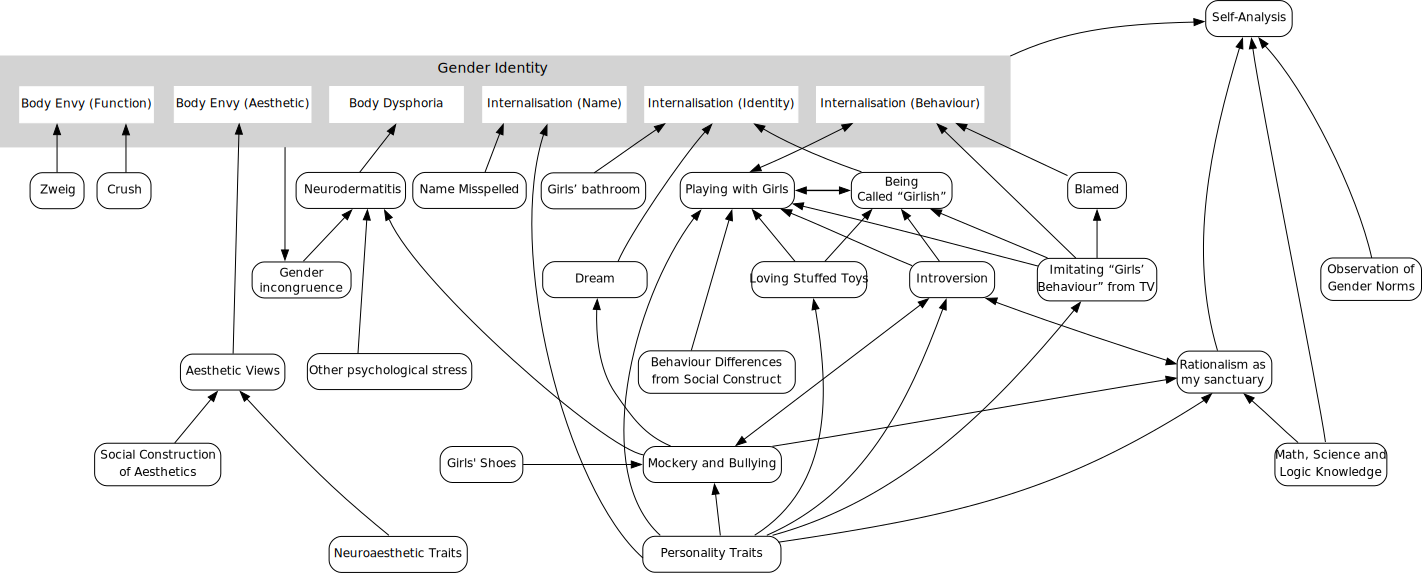
\includegraphics[width=\textwidth]{figures/bundle_of_gender_identity-simplified}
    \caption{Origins of the author's gender identity. Visualised using graphviz \parencite{Ellson2001Graphviz} and manually corrected with Inkscape \parencite{Inkscape}.\label{fig:bundle}}
\end{figure}

On the other hand, the male component is relatively simple: body representation congruence (relatively) and the externally imposed male socialisation. In particular, there is a representative anecdote worth mentioning. In a debate with gender-critical feminists, I pointed out their logical fallacies and misinterpretations of biological knowledge. They responded that "Logic is a thought of male privilege. You think like a male, so you fundamentally do not understand our female experience." In this process, I was labelled as "male," which shaped the male aspect of my self-identity. If "opposing `feminism' is a male political view" and "I oppose `feminism,'" then I updated my self-model: maybe I am "male." (This event happened about seven years ago, and I didn't know much about feminism and gender theories at that time.)

More importantly, my reliance on reason is not ``a thought of male privilege.'' My childhood experiences made me feel that the real world is chaotic and painful, while mathematics, logic, and science are beautiful. I remember very clearly when I was being bullied, how my heart raced, my legs trembled, and tears streamed down my face uncontrollably, while I insisted on telling them, ``You only hit me because your ideas are all unreasonable, because you can't win a debate against me.'' Reason has never been masculine. It is intimately intertwined with the most feminine experience of my gender identity. Reason was the only shield of that little girl in the red shoes in her most vulnerable moment. In a world full of chaos and pain, it is the only clean, pure, and trustworthy thing. It is her shield, his home, their shelter. It finally becomes an impregnable sanctuary against any irrational violence. Reason and objectivity is a long-standing tradition in feminism \parencite{Antony2018Mind}. This is the literal meaning of "enlightenment": use the light of reason to lighten all darkness. \textit{Veritas nos liberabit.}

Additionally, this model bridges the gap between the subjective experience of transgender people and social constructivism, represented by queer theory. Though I may have disagreements with post-structuralists in multiple areas, like the objectivity of science. On this particular issue, we are actually describing the same process from different perspectives and levels. Predictive coding provides a material foundation for gender performativity. It also answers the question that why gender is performative, but gender identity is subjectively so real, which Butler themself also discussed in an interview with \textcite{Williams2014Gender}. Gender identity is an acquired psychological state, but it is acquired subtly and unconsciously, and being integrated into our self-model. For an individual themself, it feels very "innate." Honestly, I also felt my gender identity very "innate" before I did the self-analysis. While I thought this is scientifically impossible, which drives me to read neurological articles. Materialist understanding liberates people from the burden of proving their validity through metaphysical claims, allowing them to view their gender identity as a functional and adaptive component of their consciousness.

\section{Conclusion}

In this paper, I have argued for a radical restructuring of how we define sex and interpret gender identity. First, I demonstrated that the concept of "phenotypic sex" is an arbitrary and unjustified subset of sexual dimorphism that begs the question; scientific precision requires us to restrict "sex" strictly to gametes and treat all other features as variable traits on a spectrum. Second, I challenged the "innate gender identity" and "brain sex" hypotheses, showing them to be incompatible with evolutionary efficiency and neuroplasticity.

Instead, I have established the predictive coding theory as a superior explanatory model. This framework posits that gender identity is constructed by the brain to minimise prediction errors caused by the friction between raw, pre-linguistic feelings (such as body incongruence, autistic sensory processing, or trauma) and enforced social categories. This model successfully bridges the gap between the biological reality of the brain and the social reality of gender constructs without falling into essentialism.

Politically, this approach disarms conservative appeals to "biological reality" by revealing the fluidity of sexual dimorphism and the cognitive mechanisms of identity formation. For transgender individuals, particularly those who are neurodivergent, this theory offers a validating, demystified self-understanding that relies on cognitive necessity rather than metaphysical souls. This model needs more positivistic studies, particularly focusing on the specific neural correlates of prediction error minimisation in atypical and non-binary transgender populations, to further substantiate these theoretical claims.

\paragraph{Declaration of interests} The author declares no competing interests.

\paragraph{Declaration of Artificial Intelligence}
Google Nano Banana Pro (gemini-3-pro-image-preview) was employed to repair my old photos (Fig. 1c, 1d), whose original versions are damaged or faded. It is strictly limited to technical restoration, and did not alter the semantic content. The original version is available for confirming their authenticity.

%\theendnotes

\printbibliography

\end{document}
